\chapter{Classificatore di Risonanze magnetiche}

\section{Problema}
La malattia di Alzheimer è una patologia neurodegenerativa progressiva che rappresenta una delle principali cause di demenza nella popolazione anziana. A causa dell’invecchiamento globale della popolazione, il numero di pazienti affetti è in costante aumento, rendendo fondamentale lo sviluppo di strumenti diagnostici affidabili e precoci.

\begin{figure}[htbp]
    \centering
    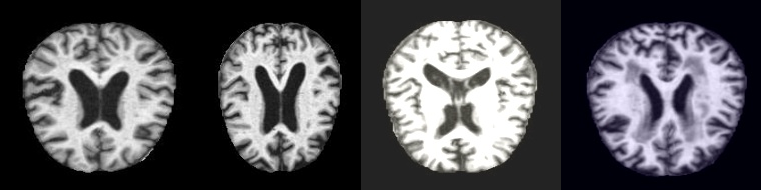
\includegraphics[width=\textwidth]{images/merged.png}
    \caption{Esempi di immagini RM (MRI) cerebrali per la classificazione dell'Alzheimer: da sinistra a destra 
    \textit{NonDemented} (assenza di demenza),
    \textit{Mild Demented} (demenza lieve), 
    \textit{Moderate Demented} (demenza moderata), 
    \textit{Very Mild Demented} (demenza molto lieve).}
    \label{fig:merged-alzheimer-mri}
\end{figure}

Il problema affrontato in questo lavoro consiste nella classificazione automatica di immagini MRI cerebrali in quattro classi, rappresentative di differenti stadi della malattia di Alzheimer (ad esempio: Non Demented, Very Mild Demented, Mild Demented, Moderate Demented). L’obiettivo è sviluppare un modello in grado di distinguere accuratamente tali classi, supportando il processo diagnostico e contribuendo a una possibile identificazione precoce della patologia.

\section{Dataset}
Il dataset utilizzato è costituito da immagini di risonanze magnetiche (MRI) celebrale ed è stato ottenuto dalla piattaforma \textbf{Kaggle}, dove è reso disponibile gratuitamente. L'acquisizione delle immagini non è resa nota nella descrizione sul sito di Kaggle. 

Ogni cartella contiene esclusivamente le immagini appartenenti alla classe corrispondente. Il dataset comprende un totale di $35.202$ immagini. L'etichettatura dei dati è \textbf{già fornita} nel dataset originale e non è stata modificata. Le immagini sono suddivise in quattro classi cliniche, organizzate in cartelle separate, in base al livello di \emph{severità} della demenza (con a seguito il numero di esempi per classe): 
\begin{enumerate}
    \item \emph{Non Demented} $12.800$
    \item \emph{Mild Demented} - $4.674$.
    \item \emph{Moderate Demented} - $6.528$.
    \item \emph{Very Mild Demented} - $11.200$.
\end{enumerate}

Le strategie utilizzate per la divisione in training set e test set variano in base al metodo impiegato per la classificazione. DA FINIRE.

\section{Metodi}
La prima parte del progetto è stata la feature extraction: abbiamo allenato diversi modelli per capire quale riusciva ad estrarre meglio le features.
\subsection{Resnet-18}
\begin{figure}[htbp]
    \centering
    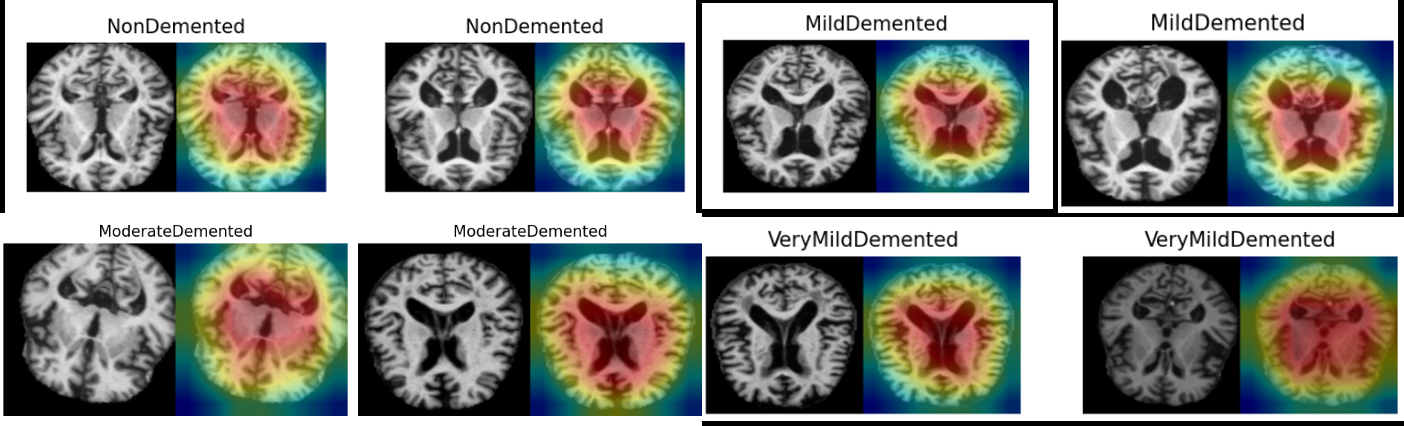
\includegraphics[width=\textwidth]{images/heatmaps-resnet18-merged.png}
    \caption{Esempi di mappe di attivazione (Grad-CAM) ottenute dal modello ResNet-18 per le quattro classi considerate: \textit{NonDemented}, \textit{MildDemented}, \textit{ModerateDemented} e \textit{VeryMildDemented}. 
    Per ciascun esempio sono mostrate l'immagine MRI originale (a sinistra) e la corrispondente heatmap sovrapposta (a destra), che evidenzia le regioni cerebrali maggiormente rilevanti per la decisione del modello. 
    Le aree in rosso indicano le zone con maggiore contributo alla classificazione.}
    \label{fig:resnet18_gradcam}
\end{figure}
Abbiamo utilizzato un modello ResNet-18 pre-addestrato su ImageNet come feature extractor. Le immagini sono state ridimensionate a $224 \times 224$ pixel per adattarsi all'input del modello. Abbamo diviso il dataset in training e test set con una proporzione dell'80\%-20\%. Dopo l'estrazione delle feature, abbiamo addestrato un classificatore Multi-Layer Perceptron (MLP) con due layer lineari e funzione di attivazione ReLU. Il modello è stato addestrato per 100 epoche con un learning rate di 0.001 e un momentum di 0.9.

\begin{table}[h!]
\centering
\begin{tabular}{lcccc}
\hline
\textbf{Classe} & \textbf{Precision} & \textbf{Recall} & \textbf{F1-score} & \textbf{Support} \\
\hline
MildDemented        & 0.79 & 0.91 & 0.85 & 919  \\
ModerateDemented   & 0.98 & 0.99 & 0.99 & 1317 \\
NonDemented        & 0.93 & 0.83 & 0.88 & 2559 \\
VeryMildDemented   & 0.84 & 0.89 & 0.86 & 2246 \\
\hline
\textbf{Accuracy}      &      &      & 0.89 & 7041 \\
\textbf{Macro Avg}     & 0.89 & 0.91 & 0.89 & 7041 \\
\textbf{Weighted Avg}  & 0.89 & 0.89 & 0.89 & 7041 \\
\hline
\end{tabular}
\caption{Classification report del modello ResNet-18.}
\label{tab:classification_report}
\end{table}

\begin{table}[h!]
\centering
\begin{tabular}{lcccc}
\hline
\textbf{True / Pred} & \textbf{Mild} & \textbf{Moderate} & \textbf{Non} & \textbf{Very Mild} \\
\hline
MildDemented        & 835 & 6   & 32  & 46  \\
ModerateDemented   & 6   & 1308 & 1   & 2   \\
NonDemented        & 97  & 5   & 2129 & 328 \\
VeryMildDemented   & 115 & 12  & 121 & 1998 \\
\hline
\end{tabular}
\caption{Confusion matrix del modello}
\label{tab:confusion_matrix}
\end{table}

\subsection{RadNet-50}
\begin{figure}[htbp]
    \centering
    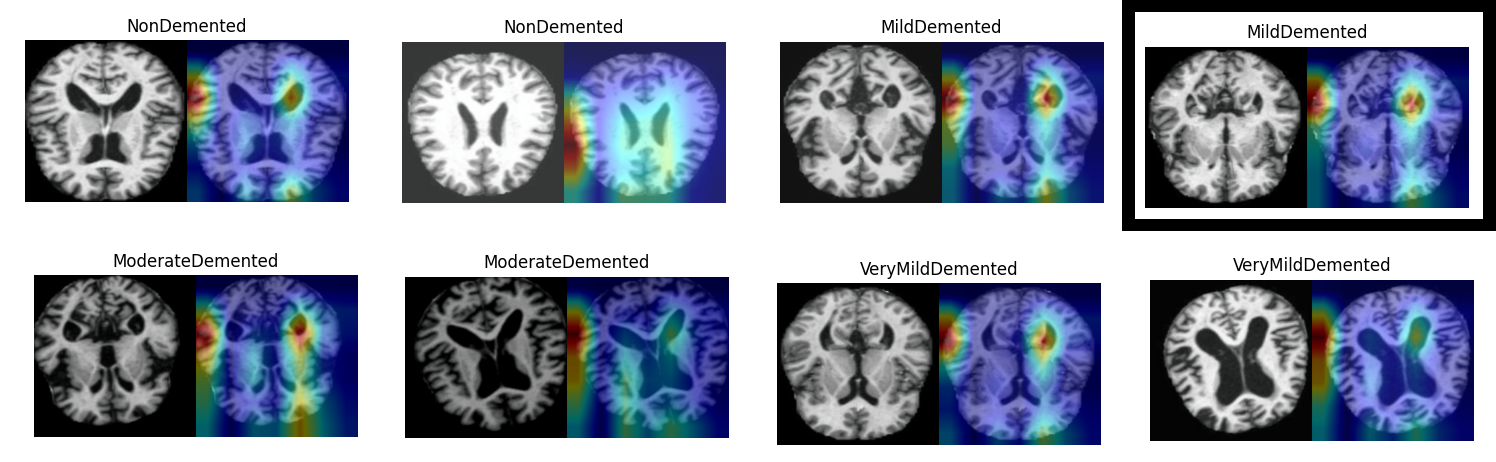
\includegraphics[width=\textwidth]{images/radnet-heatmaps-merged.png}
    \caption{Esempi di mappe di attivazione (Grad-CAM) ottenute dal modello RadNet-50 per le quattro classi considerate: \textit{NonDemented}, \textit{MildDemented}, \textit{ModerateDemented} e \textit{VeryMildDemented}. 
    Per ciascun esempio sono mostrate l'immagine MRI originale (a sinistra) e la corrispondente heatmap sovrapposta (a destra), che evidenzia le regioni cerebrali maggiormente rilevanti per la decisione del modello. 
    Le aree in rosso indicano le zone con maggiore contributo alla classificazione.}
    \label{fig:radnet_gradcam}
\end{figure}

Per migliorare le prestazioni rispetto al feature extractor ResNet-18, abbiamo utilizzato una ResNet-50 pre-addestrata su \emph{RadImageNet} (di seguito \emph{RadNet-50}), un insieme di dati radiologici che rende il backbone più adatto a domini medicali rispetto al pre-training su ImageNet. Il modello è stato impiegato come \textbf{feature extractor} e successivamente le feature sono state date in input ad un classificatore \textbf{MLP con Softmax}.

\paragraph{Pre-processing e data augmentation.}
Le immagini MRI, originariamente in scala di grigi, sono state replicate su tre canali e normalizzate con le statistiche di ImageNet. L’input del modello è stato portato a $224\times224$. Durante l’addestramento sono state applicate trasformazioni di data augmentation leggere e compatibili con il dominio MRI, al fine di migliorare la capacità di generalizzazione del modello:
\begin{itemize}
    \item ridimensionamento a $256\times256$ e \texttt{crop} (casuale in training, centrale in validazione e test);
    \item trasformazioni affini moderate (rotazioni, traslazioni e variazioni di scala);
    \item normalizzazione con media e deviazione standard di ImageNet.
\end{itemize}

\paragraph{Ottimizzazione e iperparametri principali.}
L’addestramento è stato condotto utilizzando l’ottimizzatore \textbf{AdamW} con \textbf{weight decay} pari a $10^{-4}$. Per stabilizzare il fine-tuning del modello sono stati adottati \textbf{learning rate differenziati} per le diverse parti della rete:
\begin{itemize}
    \item \textbf{head} (layer finale): $5\cdot10^{-5}$;
    \item \textbf{layer4} del backbone: $10^{-5}$;
    \item \textbf{layer3} del backbone: $5\cdot10^{-6}$.
\end{itemize}
Per ridurre l’overfitting e migliorare la stabilità dell’addestramento sono stati inoltre impiegati \textbf{dropout} (0.5) nella head, \textbf{label smoothing} (0.05), \textbf{gradient clipping} con norma massima pari a 1.0 e \textbf{mixed precision} (AMP), quando disponibile. Inoltre, per limitare la deriva del backbone durante il fine-tuning, sono stati congelati i parametri (e le statistiche delle BatchNorm) ad eccezione degli ultimi blocchi convoluzionali (\texttt{layer4} e, opzionalmente, \texttt{layer3}).

\paragraph{Estrazione delle feature e classificatore MLP.}
Una volta ottenuto il backbone ottimizzato, sono state estratte feature di dimensione 2048 (output della rete prima del layer fully connected) e usate come input di un \textbf{MLP con Softmax}. Il classificatore è stato addestrato per 50 epoche con \textbf{SGD} (learning rate 0.01, momentum 0.9) e \textbf{pesi di classe} nella loss per mitigare lo sbilanciamento del dataset.

\paragraph{Risultati (MLP su feature RadNet-50).}
Di seguito si riportano i risultati ottenuti dal classificatore MLP sulle feature estratte da RadNet-50.

\begin{table}[h!]
\centering
\begin{tabular}{lcccc}
\hline
\textbf{Classe} & \textbf{Precision} & \textbf{Recall} & \textbf{F1-score} & \textbf{Support} \\
\hline
MildDemented        & 0.58 & 0.18 & 0.28 & 935  \\
ModerateDemented   & 0.68 & 0.97 & 0.80 & 1306 \\
NonDemented        & 0.71 & 0.59 & 0.65 & 2560 \\
VeryMildDemented   & 0.49 & 0.60 & 0.54 & 2240 \\
\hline
\textbf{Accuracy}     &      &      & 0.61 & 7041 \\
\textbf{Macro Avg}    & 0.61 & 0.58 & 0.56 & 7041 \\
\textbf{Weighted Avg} & 0.62 & 0.61 & 0.59 & 7041 \\
\hline
\end{tabular}
\caption{Classification report del classificatore MLP addestrato sulle feature estratte con RadNet-50.}
\label{tab:radnet_mlp_best_report}
\end{table}

\begin{table}[h!]
\centering
\begin{tabular}{lcccc}
\hline
\textbf{True / Pred} & \textbf{Mild} & \textbf{Moderate} & \textbf{Non} & \textbf{Very Mild} \\
\hline
MildDemented        & 169 & 135 & 43  & 588 \\
ModerateDemented   & 9   & 1262 & 1   & 34  \\
NonDemented        & 35  & 212 & 1521 & 792 \\
VeryMildDemented   & 77  & 240 & 584 & 1339 \\
\hline
\end{tabular}
\caption{Confusion matrix del classificatore MLP su feature RadNet-50.}
\label{tab:radnet_mlp_best_cm}
\end{table}

L'approccio è stato in generale fallimentare, probabilmente a causa della natura specifica delle immagini MRI che richiedono un fine-tuning più approfondito del backbone. Tuttavia, l'analisi delle mappe di attivazione (Figura \ref{fig:radnet_gradcam}) mostra che il modello non è in grado di focalizzarsi sulle regioni cerebrali rilevanti, suggerendo la necessità di un addestramento più mirato.

\subsection{Custom-CNN}
\begin{figure}[htbp]
    \centering
    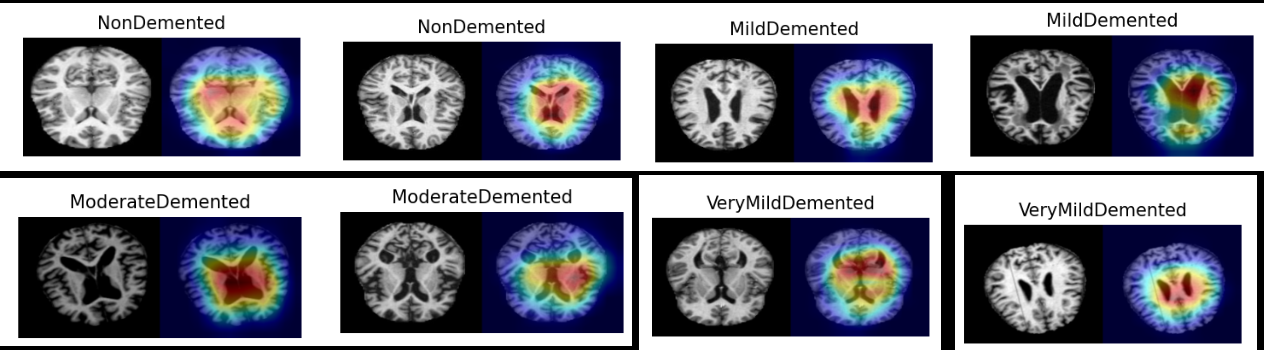
\includegraphics[width=\textwidth]{images/custom-cnn-heatmaps.png}
    \caption{Esempi di mappe di attivazione (Grad-CAM) ottenute dal modello Custom-CNN per le quattro classi considerate: \textit{NonDemented}, \textit{MildDemented}, \textit{ModerateDemented} e \textit{VeryMildDemented}. 
    Per ciascun esempio sono mostrate l'immagine MRI originale (a sinistra) e la corrispondente heatmap sovrapposta (a destra), che evidenzia le regioni cerebrali maggiormente rilevanti per la decisione del modello. 
    Le aree in rosso indicano le zone con maggiore contributo alla classificazione.}
    \label{fig:custom_cnn_gradcam}
\end{figure}

Per migliorare ulteriormente le performance del classificatore, abbiamo progetto e implementato una CNN personalizzata. 

\paragraph{Architettura.}
L'architettura della rete è ispirata all'architettura della ResNet-18, in totale è composta da 14 layer ed è divisa da:
\begin{itemize}
    \item \textbf{Fase di inizializzazione}: Questda parte è composta da un layer convoluzione che serve per ridurre la dimensione dell'immagine di input di dimensione $1 \times 176 \times 208$ e lo converte in un tensore di dimensione $32 \times 88 \times 104$, seguito da un layer di batch normalization e una funzione di attivazione ReLU. Successivamente, un layer di max pooling che riduce la dimensione a $32 \times 44 \times 52$.
    \item \textbf{Tre basic blocks}: ciascun blocco contiene due layer convoluzionali seguiti da operazioni di batch normalization e funzioni di attivazione ReLU. Alla fine c'è un layer chiamato \emph{shortcut} che serve nella fase di backpropagation per evitare il problema del vanishing gradient, per mezzo di un altro layer convoluzionale con kernel di dimensione $1 \times 1$ e un layer di batch normalization.
    \item \textbf{Average Pooling}: un layer di average pooling che riduce ulteriormente la dimensione del tensore a $128 \times 1 \times 1$.
    \item \textbf{Layer lineare}: un layer lineare che mappa le feature estratte alle quattro classi di output, con un dropout del 25\%.
\end{itemize}

L'estrazione di feature è stata effettuata utilizzando l'intera rete, addestrata da zero dividendo il dataset in training e test set con una proporzione dell'80\%-20\%. Per ottimizzare il modello è stato utilizzato ADAM (Adaptive Moment Estimation), è stato preferito perché è in grado di adattarsi avendo un learning rate dinamico durante l'addestramento e convergere più velocemente rispetto alla discesa del gradiente standard. Il modello è stato poi addestrato per 20 epoche con un learning rate di 0.001. Modificando l'ultimo layer trasformandolo in un MLP con Softmax, abbiamo ottenuto i seguenti risultati sul test set:
\begin{table}[h!]
\centering
\begin{tabular}{lcccc}
\hline
\textbf{Classe} & \textbf{Precision} & \textbf{Recall} & \textbf{F1-score} & \textbf{Support} \\
\hline
MildDemented        & 0.96 & 0.98 & 0.97 & 919  \\
ModerateDemented   & 1.00 & 1.00 & 1.00 & 1317 \\
NonDemented        & 0.96 & 0.95 & 0.95 & 2559 \\
VeryMildDemented   & 0.95 & 0.95 & 0.95 & 2246 \\
\hline
\textbf{Accuracy}     &      &      & 0.96 & 7041 \\
\textbf{Macro Avg}    & 0.97 & 0.97 & 0.97 & 7041 \\
\textbf{Weighted Avg} & 0.96 & 0.96 & 0.96 & 7041 \\
\hline
\end{tabular}
\caption{Classification report del modello finale}
\label{tab:classification_report_final}
\end{table}

\begin{table}[h!]
\centering
\begin{tabular}{lcccc}
\hline
\textbf{True / Pred} & \textbf{Mild} & \textbf{Moderate} & \textbf{Non} & \textbf{Very Mild} \\
\hline
MildDemented        & 904 & 0   & 5    & 10   \\
ModerateDemented   & 0   & 1317 & 0    & 0    \\
NonDemented        & 17  & 1   & 2428 & 113  \\
VeryMildDemented   & 23  & 0   & 96   & 2127 \\
\hline
\end{tabular}
\caption{Confusion matrix del modello finale}
\label{tab:confusion_matrix_final}
\end{table}

\section{Valutazione}
Per una valutazione a $K=4$ classi ($c \in \{1, 2, 3, 4\}$), sia $C$ la matrice di confusione $4 \times 4$, dove $C_{i, j}$ rappresenta il numero di campioni con classe $I$ che sono stati classificati come classe $j$. Definiamo:
\begin{align*}
&TP_k = C_{k,k} \\
&FP_k = \sum_{i=1, i \neq k}^{4} C_{i,k} \\
&FN_k = \sum_{i=1, i \neq k}^{4} C_{k,i} \\
&TN_k = \sum_{i=1}^{4} \sum_{j=1}^{4} C_{i,j} - TP_k - FP_k - FN_k
\end{align*}

Le metriche utilizzate per valutare le performance del modello sono:
\begin{itemize}
    \item \textbf{Precision}: misura la proporzione dei veri positivi rispetto al totale dei positivi predetti dal modello.
    \[
    \text{precision}_k = \frac{TP_k}{TP_k + FP_k}
    \]
    \item \textbf{Recall}: misura la proporzione dei veri positivi rispetto al totale dei positivi effettivi nel dataset.
    \[
    \text{recall}_k = \frac{TP_k}{TP_k + FN_k}
    \]
    \item \textbf{F1-score}: è la media armonica tra precision e recall, fornendo una misura bilanciata delle performance del modello.
    \[
    \text{F1-score}_k = 2 \cdot \frac{\text{precision}_k \cdot \text{recall}_k}{\text{precision}_k + \text{recall}_k}
    \]
    \item \textbf{Support}: il numero di occorrenze di ogni classe nel dataset di test.
    \[
    \text{support}_k = \sum_{i=1}^{4} C_{k,i}
    \]
\end{itemize}

\section{Demo}

\section{Codice}

\section{Conclusioni}